\chapter{Método de Trabajo}
\label{chap:metodo}
\label{chap:metodologia}

%haz un check de los acrónimos

\section{\acf{PUD}}

\drop{E}{n} \cite{rumbaugh_jacobson_pud} se define el \acf{PUD} como un proceso de desarrollo
de software. A su vez, un proceso de desarrollo de software es el conjunto de
actividades necesarias para transformar los requisitos de usuario en un sistema
software (véase figura \ref{fig:proc-software}). 

\begin{figure}[!h]
  \begin{center}
    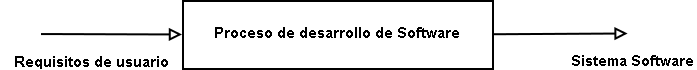
\includegraphics[width=1.0\textwidth]{/proceso-software.png} 
    \caption{Proceso Software \cite{rumbaugh_jacobson_pud}}
    \label{fig:proc-software}
  \end{center}
\end{figure}


El \acs{PUD} está basado en \textit{componentes}, lo que significa que el
software en construcción está formado por componentes interconectados a través de
interfaces bien definidas. 

Para diseñar y desarrollar todos los artefactos de un sistema software, el \acs{PUD}
utiliza un lenguaje unificado de desarrollo denominado \acf{UML}. Se puede consultar más información sobre \acs{UML} en \cite{rumbaugh_unified_2004}. 

\cite{rumbaugh_jacobson_pud} define las principales características del
\acs{PUD} en: 

\begin{enumerate}
\item Dirigido por casos de uso.
\item Centrado en la arquitectura.
\item Iterativo e incremental.
\end{enumerate}

\subsection{Características del Proceso Unificado de Desarrollo}

\subsubsection{Dirigido por casos de uso}

La finalidad de un sistema software es proporcionar servicio a los usuarios
\cite{rumbaugh_jacobson_pud}. Estos usuarios pueden ser tanto humanos como otros
sistemas, luego el término \textit{usuario} se refiere a toda aquella entidad
que interactúa con el sistema que se está desarrollando. Es una interacción
concreta la que da nombre al concepto \acf{CdU}.

En \cite{rumbaugh_jacobson_pud} se define \textbf{caso de uso} como un fragmento
de funcionalidad del sistema que proporciona al usuario un resultado
importante. 

La función de los casos de uso es representar los requisitos funcionales del
sistema. Al conjunto de todos los casos de uso se le denomina \textbf{modelo de
  casos de uso}. \cite{rumbaugh_jacobson_pud} define al modelo de casos de uso
a aquel formado por casos de uso, actores y sus relaciones. Un modelo de casos de
uso define la funcionalidad de todo el sistema, así pues representa todos los
escenarios de interacción posible entre el usuario y el sistema. 

\cite{rumbaugh_jacobson_pud} advierte que si bien es cierto que los casos de uso
guían el proceso no deben ser desarrollados de manera aislada, pues hay que
considerar la arquitectura del sistema. \textit{Los casos de uso guían la
  arquitectura del sistema y la arquitectura del sistema influye en la selección
  de los casos de uso}. 

Esto sugiere que existe un proceso de \textbf{maduración} tanto de arquitectura
como del modelo de casos de uso a medida que avanza el ciclo de desarrollo. 
 

\subsubsection{Centrado en la arquitectura}

Al igual que en la construcción de edificios, el papel de la arquitectura de
software se puede contemplar desde diversos puntos de vista, tales como
estructura o servicios \cite{rumbaugh_jacobson_pud}. En una arquitectura
software la visión incluye aspectos estáticos y dinámicos. Así pues una
arquitectura surge de las necesidades y refleja los casos de uso, pero también
se ve influida por otros muchos factores (plataforma, marcos de trabajo,
interfaces gráficas, requisitos de rendimiento o fiabilidad, etc.). 

\cite{rumbaugh_jacobson_pud} denota que la relación existente entre casos de uso
y arquitectura debe ser la siguiente: 

\begin{enumerate}
\item Los casos de uso deben encajar en la arquitectura cuando se llevan a cabo.

\item La arquitectura debe permitir el desarrollo de todos los casos de uso
  requeridos y permitir una evolución en paralelo. 
\end{enumerate}

De esta manera los casos de uso representan la función del sistema mientras que
la arquitectura define la forma de dicho sistema.

Según \cite{rumbaugh_jacobson_pud} el arquitecto:

\begin{enumerate}

\item Realizará una versión inicial de la arquitectura, comenzando por la sección del
  sistema que no es específica de los casos de uso pero debe mantener en
  perspectiva de éstos antes de comenzar la creación del esquema arquitectónico.

\item Trabajará con un subconjunto de los casos de uso que represente las
  funciones clave del sistema. Estos casos de uso deben especificarse en detalle y
  se realizará en términos de subsistemas, clases y componentes. 

\item A medida que los casos de uso se especifican y desarrollan se
  descubren nuevos aspectos de la arquitectura, lo que implica una maduración de
  los casos de uso. 

\end{enumerate}


\subsubsection{Iterativo e incremental}

Cuando se aborda el desarrollo de un producto software se asume que supondrá un
gran esfuerzo en términos económicos y temporales. Así pues resulta práctico
dividir el trabajo en partes más pequeñas que se denominan iteraciones. Cada
iteración obtendrá como resultado un incremento y dicho incremento se traducirá
en una pequeña mejora o avance en el desarrollo del producto. En
\cite{rumbaugh_jacobson_pud} se remarca la necesidad de establecer iteraciones
\textit{controladas}, es decir, iteraciones que deben ser previamente
seleccionadas y ejecutadas de forma planificada como si fuesen proyectos más
pequeños. 

Para llevar a cabo este control, el desarrollador basa la selección en dos
factores \cite{rumbaugh_jacobson_pud}: 

\begin{enumerate}
\item La iteración tratará un grupo de casos de uso que en conjunto ampliarán la
  utilidad del producto desarrollado. 
\item La iteración tratará los riesgos más importantes. 
\end{enumerate}

Puesto que cada iteración se considera un mini-proyecto, tomarán como punto de
partida los casos de uso y después desarrollará el trabajo según  los flujos: 

\begin{enumerate}
\item Análisis
\item Diseño
\item Implementación
\item Pruebas
\end{enumerate}

\cite{rumbaugh_jacobson_pud} aclara que al final de cada iteración no se tiene
por qué tener un incremento necesariamente aditivo puesto que en las primeras
fases del ciclo de vida los desarrolladores pueden tener que realizar tareas de
reemplazo de diseño (los más superficiales por los más sofisticados). No
obstante en las fases posteriores los incrementos suelen ser aditivos. 

Según \cite{rumbaugh_jacobson_pud}  el desarrollador durante una iteración del
\acs{PUD} debe realizar las siguientes tareas: 

\begin{enumerate}
\item Identificar y especificar los casos de uso más relevantes. 
\item Crear un diseño siguiendo la arquitectura seleccionada. 
\item Implementar el diseño mediante componentes. 
\item Verificar que los componentes satisfacen los casos de uso. 
\end{enumerate}

Todo ello ciñéndose al orden lógico de las iteraciones para economizar recursos
y lograr el objetivo. Es habitual que surjan problemas inesperados y sea
necesario realizar adaptaciones a los nuevos problemas, pero siguiendo un plan
los beneficios son significativos:


\begin{enumerate}
\item El coste del riesgo se reduce a solo un incremento del proceso. Si una
  iteración debe repetirse, la organización sólo perdería el esfuerzo empleado
  en la iteración en concreto. 
\item Se reduce el riesgo de retrasos en la entrega del producto mediante la
  identificación de riesgos en las fases más tempranas. 
\item Puesto que los desarrolladores trabajan de manera más eficiente se
  consigue incrementar el ritmo del esfuerzo de desarrollo. 
\item El cambio de requisitos por parte de los usuarios no es acentuado, debido
  a que los requisitos se van refinando durante las iteraciones. 
\end{enumerate}


\subsection{Ciclo de vida del Proceso Unificado de Desarrollo}

\subsubsection{Modelo del \acs{PUD}}

El \acs{PUD} se repite a lo largo de una serie de ciclos que constituyen la vida
de un sistema y cada ciclo concluye con una versión del producto
\cite{rumbaugh_jacobson_pud}. 

Cada ciclo está constituido por cuatro fases y cada fase a su vez se divide en
iteraciones como ilustra la figura \ref{fig:ciclos-pud}.  


\begin{figure}[!h]
  \begin{center}
    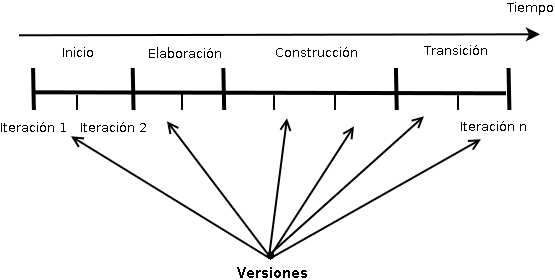
\includegraphics[width=0.8\textwidth]{/ciclos.png} 
    \caption{Ciclo con fases e iteraciones \cite{rumbaugh_jacobson_pud}.}
    \label{fig:ciclos-pud}
  \end{center}
\end{figure}


En cada ciclo se produce una nueva versión del sistema, siendo una versión un
producto preparado para su entrega. El entregable a su vez consta de un cuerpo
de código fuente además de manuales y productos asociados a su
funcionamiento. El producto terminado incluirá los requisitos, casos de uso,
especificaciones no funcionales y casos de prueba, incluyendo el modelo de la
arquitectura y el visual. 


Para llevar a cabo los ciclos del \acs{PUD} los desarrolladores necesitan todas las
representaciones del producto software. Estas representaciones del producto se
denominan \textbf{Modelo del Proceso Unificado} (véase figura \ref{fig:ciclo-fin}).

\begin{figure}[!h]
  \begin{center}
    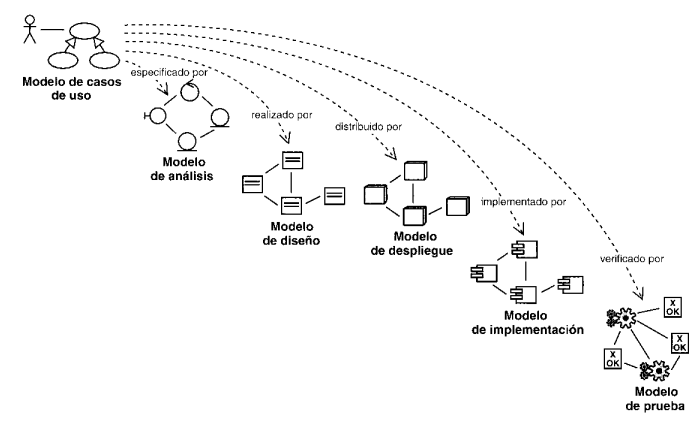
\includegraphics[width=0.8\textwidth]{/ciclofin.png} 
    \caption{Modelo del \acs{PUD} extraído de \cite{rumbaugh_jacobson_pud}.}
    \label{fig:ciclo-fin}
  \end{center}
\end{figure}


\begin{itemize}
\item \textbf{Modelo de casos de uso}: Todos los casos de uso del producto
  software. 
\item \textbf{Modelo de análisis}: Refina los casos de uso añadiendo más
  detalles y asigna funcionalidad a los objetos del producto software que
  proporcionan comportamiento.
\item \textbf{Modelo de diseño}: Define la estructura estática del sistema
  (subsistemas, clases e interfaces) que representan los casos de uso. 
\item \textbf{Modelo de implementación}: Incluye los componentes, que
  representan al código fuente así como la correspondencia entre las clases y
  esos dichos componentes.
\item \textbf{Modelo de despliegue}: Define los nodos físicos y su
  correspondencia con los componentes.
\item \textbf{Modelo de prueba}: Especifica los casos de prueba que verifican
  los casos de uso.
\item \textbf{Representación de la arquitectura}: Una representación de la
  arquitectura del sistema software desarrollado. 
\item El sistema debe tener un modelo de dominio o modelo del negocio. Su
  objetivo es describir el contexto del negocio en el que se encuentra el
  sistema. 
\end{itemize}


\subsubsection{Fases de un ciclo del Proceso Unificado de Desarrollo}

\cite{rumbaugh_jacobson_pud} cita y explica las cuatro fases de cada ciclo del \acs{PUD}:

\begin{enumerate}
\item Inicio
\item Elaboración
\item Construcción 
\item Transición
\end{enumerate}

A su vez, cada fase se puede descomponer a su vez en
iteraciones (véase figura \ref{fig:fases-ciclo}), acabando cada iteración en un hito. En la siguiente figura se
representa el esfuerzo que se realiza en cada una de las fases. 


\begin{figure}[!h]
  \begin{center}
    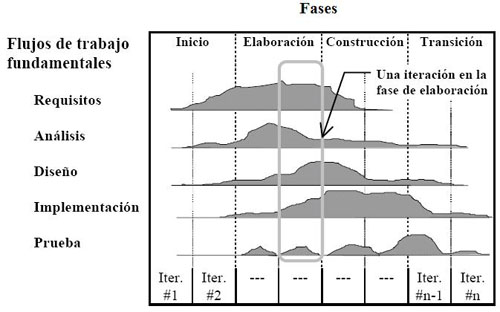
\includegraphics[width=0.8\textwidth]{/fases.jpg} 
    \caption{Diferentes fases del \acs{PUD} \cite{rumbaugh_jacobson_pud}.}
    \label{fig:fases-ciclo}
  \end{center}
\end{figure}



\textbf{Fase de Inicio}: En la fase de inicio se realiza una descripción del
producto final, es decir, se realiza el análisis de negocio para el producto
esperado. En esta fase se responde a las siguientes cuestiones: 

\begin{itemize}
\item Cuáles son las principales funciones del sistema para sus usuarios más
  importantes: lo que dará como resultado el modelo de casos de uso
  simplificado, conteniendo aquellos más críticos. 
\item Cómo podría ser la arquitectura del sistema: una vez se tiene el modelo,
  se comienza a esbozar la arquitectura con los subsistemas más importantes.

\item Cuál es el plan de proyecto y cuánto costará desarrollar el producto: del
  paso anterior se planifican los riesgos y comienza a estimarse el coste del
  proyecto. 
\end{itemize}


\textbf{Fase de Elaboración}: En esta fase se describe con más de talle los
casos de uso y se diseña de manera definitiva la arquitectura y el sistema al
completo. Finalmente, el director del proyecto debe ser capaz de planificar las
actividades y estimar los recursos necesarios para terminar el proyecto. 

\textbf{Fase de Construcción}: Fase de desarrollo del producto. El producto
final contiene todos los casos de uso que se han acordado para el sistema. La
línea base crecerá hasta convertirse en el sistema al completo. Se tiene una
arquitectura estable pero aún susceptible de mejorar. Puede no estar
completamente libre de defectos, que serán detectados y atajados en la fase de
transición. 

\textbf{Fase de Transición}: Corresponde al periodo en el cual el producto pasa
a ser una versión \textit{beta}. Se corrigen problemas y se realizan mejoras del
sistema. Además esta fase contiene otras actividades complementarias, tales
como formación del cliente, ayuda y asistencia, soporte técnico y corrección de
defectos. Estos defectos se pueden dividir en dos categorías: 

\begin{enumerate}
\item Los que tienen suficiente impacto para justificar un incremento. 
\item Los que pueden corregirse en una versión usual. 
\end{enumerate}



\section{Planificación del Proyecto}

En esta sección se muestra la planificación que se llevará a cabo en la
realización del \acs{TFM}. En el Capítulo \ref{chap:resultados} se detallarán
todos los productos resultantes de cada una de las iteraciones. 

El sistema software a desarrollar se describe a continuación. 

\subsection{SparkDQ: Un stack de Spark para la evaluación de la calidad de datos
  de triplas semánticas} 

Este capa software tendrá por objetivo resolver el problema del tratamiento de
datos semánticos en entornos Big Data. Se integrará e interactuará con el
framework Apache Spark para ofrecer un conjunto de primitivas de lectura de
datos semánticos y evaluación de la calidad de los mismos.

Este artefacto software tendrá las siguientes responsabilidades:

\begin{itemize}
\item Permitir la lectura de triplas semánticas y almacenarlas en una estructura
  de datos conveniente de forma distribuida.
\item Evaluación de los niveles de calidad de datos de un conjunto \acs{LOD}
  para la dimensión de calidad \textit{Completeness} desde la perspectiva de dos
  de sus métricas, descritas en su sección correspondiente del capítulo 3 (\ref{metricasdq}):
  \begin{itemize}
  \item \textit{Interlinking Completeness}
  \item \textit{Schema Completeness}
  \end{itemize}
\end{itemize}

\subsection{Prueba de Concepto para SparkDQ}

Para materializar el stack elaborado en el punto anterior, se elaborará una
aplicación software que aproveche las métricas implementadas en un caso de uso
real, en el que se tendrá una perspectiva \textit{end to end} de un problema de
calidad de datos, persiguiendo los siguientes objetivos:

\begin{enumerate}
\item Ingesta de datos semánticos en un entorno Big Data.
\item Evaluación de la calidad de los datos ingestados de manera distribuida. 
\item Almacenamiento de resultados de la evaluación.
\item Consumo de los resultados de la evaluación. 
\end{enumerate}

\subsection{Requisitos funcionales para SparkDQ}
\subsection{Requisitos funcionales para la PoC}
\subsection{Iteraciones del \acs{PUD}}

\section{Marco tecnológico de trabajo}

\subsection{Frameworks de desarrollo}
\subsection{Software de desarrollo}
\subsection{Edición}
\subsection{Servidores}
\subsection{Lenguajes de programación}
\subsection{Equipos de desarrollo}

Para la realización del \acs{TFM} se han utilizado las siguientes máquinas: 

\begin{itemize}
\item PC con \textit{Microsoft Windows 7 Professional} procesador Intel Centrino
  doble núcleo de 2.1 GHz y 4 GB de RAM. 
\item PC con \textit{Debian 7 Wheezy} con procesador Intel Atom doble núcleo de
  1.2GHz y 2 GB de RAM. 
\end{itemize}
